% =====================================================================
% VERSION ENSAE, REDUCTION SFE : introduction.
% Phase 3 : copie de l'ancienne sous-section 1.5.3 (chapitres/02b_cadre_cyber_dora.tex,
% lignes 684 a 743). Phase 4 (1er octobre 2026) : reecrite selon la regle n°2 de la mission, et
% completee de ce que les consignes MS demandent a une introduction (situer le stage, le
% probleme, le contexte et les moyens employes), avec des faits pris dans le chapitre du stage,
% le chapitre 1 et la cartographie des sources du chapitre 3. Rapport :
% reduction/chapitres/00_introduction.md.
% Reprise le 1er octobre 2026 tard le soir, demande de Kelian (« une ecriture plus humaine ») :
% registre cale sur six memoires d'actuariat publies avant 2022 (style/registre_humain.py,
% style/registre_humain.md) : phrases plus longues et plus variees, connecteurs et « nous » des
% memoires de reference, moins de points-virgules et de verbes « porter ». Fond inchange.
% Lu par main_ensae.tex seul : ne jamais le faire lire par main_institut.tex.
% Le script 74 est cite pour le bruit de simulation de l'ecart (± 734 M€), publie au chapitre 10.
% =====================================================================

\chapter*{Introduction}
\phantomsection
\addcontentsline{toc}{chapter}{Introduction}
\markboth{Introduction}{}
\label{subsec:problematique-positionnement}
% SOURCES-SCRIPTS: 43 68 92 74 33 65 67 30 134 117

Le règlement européen sur la résilience opérationnelle numérique (DORA), applicable depuis $2025$,
organise les exigences de résilience informatique des entités financières autour de cinq domaines,
appelés ici piliers. Il rend observable un niveau de maîtrise que le calcul prudentiel ignore. Dans
la Formule Standard de Solvabilité~II, la charge de risque opérationnel ne dépend que de grandeurs
de volume : deux entités de même volume reçoivent la même charge quel que soit leur
état de conformité (\S\ref{subsec:critique-formule-standard}). La question étudiée est donc la
suivante : \emph{comment la distribution des pertes informatiques d'une entité, puis son besoin de
capital, varient-ils lorsque son état de conformité aux cinq piliers se dégrade ?}

La contribution est de calculer un écart de capital entre états supposés, puis d'examiner ce qui
en subsiste lorsque le sens de la contagion et les coûts par pilier ne sont pas observés.
Les lois de fréquence et de pertes, les cascades et l'identification partielle viennent de la
littérature. Leur adaptation aux domaines de contrôle et l'analyse de leurs limites constituent
l'apport du travail, précisé au chapitre~\ref{ch:positionnement}. Le modèle compare des scénarios
et précise les données manquantes ; il ne valide pas un capital d'entité.
La figure~\ref{fig:architecture-memoire} relie données, agrégation, identification et décision.

\begin{figure}[tbp]\centering
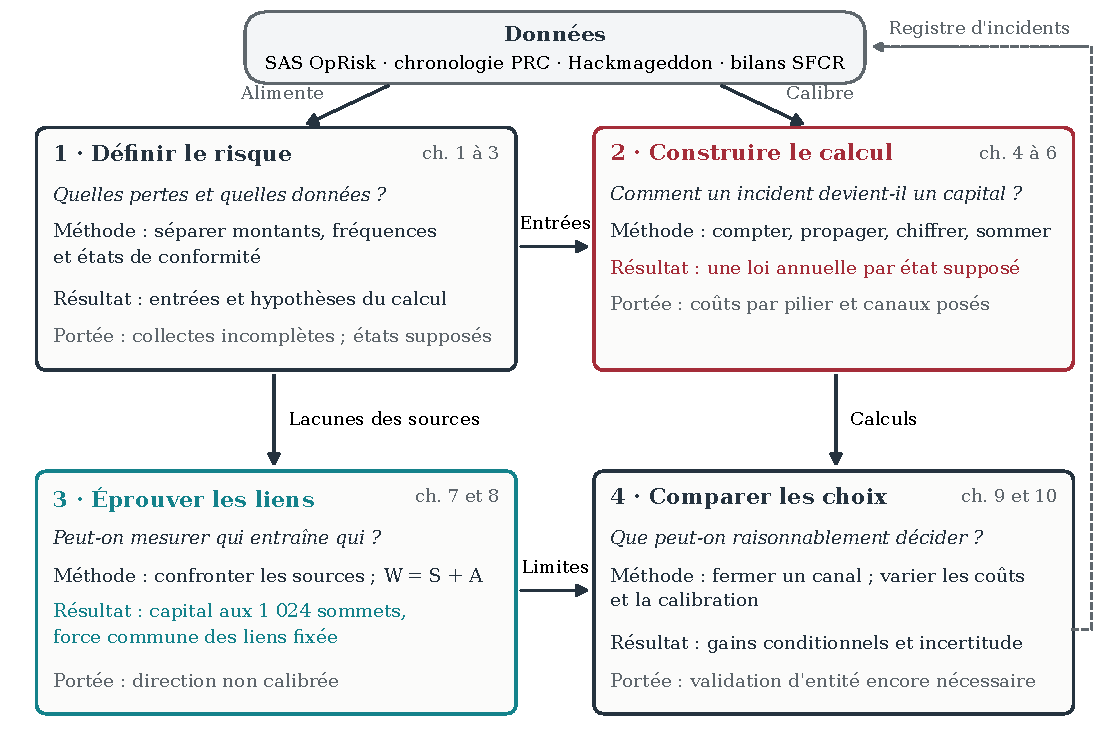
\includegraphics[width=0.9\textwidth]{figures_pedagogie/architecture_memoire.pdf}
\caption{Le fil du mémoire : une question, une méthode et un résultat transmis à la suite.
Les limites indiquent ce que chaque étape laisse à établir. Le registre proposé au
chapitre~\ref{ch:robustesse} renseignerait les entrées manquantes ; la
figure~\ref{fig:lecture-architecture} détaille le calcul annuel.}
\label{fig:architecture-memoire}
\end{figure}

Les pertes modélisées sont celles du risque opérationnel d'origine
informatique de l'entité ; les pénalités réglementaires et le risque des polices cyber qu'un
assureur vend ne sont pas modélisés. La Value-at-Risk (VaR) est le plus petit montant que la perte ne dépasse pas avec la probabilité choisie. Le capital de solvabilité requis (SCR) est une VaR à $99{,}5\,\%$ de la variation des fonds propres de base sur un an ; nous en retenons un substitut,
le quantile à $99{,}5\,\%$ de la charge annuelle de pertes.

Faute de module DORA dans la Formule
Standard, le quantile retenu est un besoin de capital au sens de l'évaluation interne des risques et de la solvabilité (ORSA), non un SCR réglementaire. Les montants sont exprimés en millions d'euros (M\euro), les actifs sources en millions de dollars (M\$).

Le calcul suit une année d'incidents. Leur nombre est tiré selon une loi binomiale négative, puis
le pilier sur lequel chacun commence. La propagation détermine les autres piliers touchés. Pour
chacun d'eux, une perte est tirée, de loi de Pareto généralisée au-delà d'un seuil ; les pertes
sont additionnées par incident, puis sur l'année.
Une année simulée peut ainsi compter trois incidents, dont l'un, parti de la gestion des
prestataires tiers, atteint ensuite la gouvernance puis la gestion des incidents. Cet incident
compte une fois dans le nombre annuel, mais sa perte additionne celles des trois piliers touchés.

Nous suivons ce même exemple aux figures~\ref{fig:lecture-architecture} et~\ref{fig:lecture-incident},
puis au \S\ref{sec:institut-unite-perte}. Le calcul est répété sur un grand nombre d'années simulées pour estimer ce quantile annuel (méthode de Monte-Carlo). La conformité modifie les paramètres de fréquence,
de détection, de propagation et de choc commun ; une chaîne de Markov décrit séparément son
évolution sur plusieurs années.

\begin{samepage}
SAS OpRisk Global fournit les pertes et les nombres d'incidents. La base \emph{Privacy Rights
Clearinghouse} (PRC) sert à comparer fréquence et sévérité. Les parts par vecteur d'Hackmageddon
pondèrent le multiplicateur de fréquence entre états. Trois résultats en découlent.\par
\end{samepage}

\begin{enumerate}[leftmargin=*,nosep]
\item \emph{Un écart de capital entre états de conformité} (chapitres~\ref{chap:cascade} à~\ref{chap:resultats}). L'état de conformité agit par quatre canaux : fréquence des incidents,
dépassement du seuil de sévérité, propagation et accumulation par un prestataire commun ; les
valeurs de ces canaux sont posées pour chaque état. Pour le périmètre financier étudié, le besoin
passe alors de $6\,049$ à $20\,188$~M\euro{}, soit un facteur $3{,}34$, et l'écart de
$14\,139$~M\euro{} présente un écart-type de $734$~M\euro{} entre quatre graines. Ces montants
comparent deux états supposés ; leur amplitude dépend des paramètres posés et de l'addition des
coûts entre piliers. À l'échelle d'une entité, fréquence et pertes sont
lues à sa taille ; l'effet du métier n'est pas estimé.
\item \emph{Une direction non identifiable} (chapitre~\ref{ch:identifiabilite}). Sur les trois sources agrégées, le sens des liens entre piliers
n'est pas identifiable ; le corpus de rapports post-incident n'en
donne qu'un ordre partiel.
\item \emph{Une plage de capital sur les directions admissibles} (chapitre~\ref{chap:partielle}). La force commune des liens est
posée à dire d'expert, et leur sens varie dans un ensemble admissible. Aux $1\,024$ sommets de cet
ensemble, le capital du calage de référence va de $6\,858$ à $8\,697$~M\euro{} (écart-type de la
largeur : $189$~M\euro{} entre quatre graines). Cette plage, conditionnelle à la force posée, n'est
ni une borne globale démontrée ni un intervalle de confiance. Documenter le sens des six
dépendances décrites par les rapports post-incident la réduirait de $32{,}7\,\%$ en moyenne, de
$22$ à $44\,\%$ selon la graine (\S\ref{ch:livrable}).
\end{enumerate}

Ce travail a été mené chez Nexialog Consulting, de juin à novembre $2026$, sous la direction de Hugo
Rapior. Les choix de modélisation relèvent de l'auteur ; l'usage de l'IA est décrit en annexe~\ref{ann:ia}.
